\documentclass{standalone}
\usepackage{tikz}
\usepackage{pgfplots}
\pgfplotsset{compat=newest}
\usepackage{amsmath}
\usepackage[american]{circuitikz}
\usepackage{cmbright}

\definecolor{myred}{RGB}{170,0,0}
\definecolor{myblue}{RGB}{0,0,220}
\definecolor{mygreen}{RGB}{0,150,0}
\definecolor{myorange}{RGB}{255,127,0}
\definecolor{mybrown}{RGB}{150,75,0}

\begin{document}
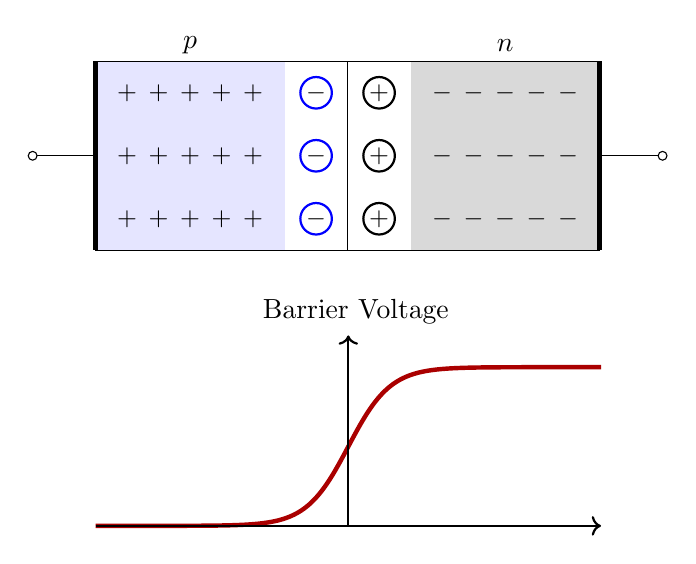
\begin{tikzpicture}
    \begin{scope}[scale=0.8]
        % Regions
        % p-region
        \fill[blue!10] (0,0) rectangle (3,3);
        % Depletion region
        \fill[white] (3,0) rectangle (5,3);
        % n-region
        \fill[gray!30] (5,0) rectangle (8,3);
        \draw[thin, black] (0, 0) rectangle (8, 3);

        % Line at the interface.
        \draw[thin, black] (4, 3) -- (4, 0);

        % Metal contact lines
        \draw[ultra thick, black] (0,3) -- (0,0);
        \draw[ultra thick, black] (8,3) -- (8,0);
        \draw[thin, black] (-1, 1.5) -- (0, 1.5);
        \draw[thin, black] (9, 1.5) -- (8, 1.5);

        % Contact terminals.
        \draw (-1, 1.5) node[ocirc] (A) {};
        % \draw (A) node[right, yshift=3mm] {$n_A$};
        \draw (9, 1.5) node[ocirc] (B) {};
        % \draw (B) node[right, yshift=-3mm] {$n_B$};

        % Charges in p-region
        \foreach \x in {-3.5,-3.0, -2.5, -2.0, -1.5} {
            \foreach \y in {0.5, 1.5, 2.5} {
                \node at (\x + 4,\y) {\small$+$};
            }
        }
        \node at (1.5, 3.25) {$p$};

        % Charges in n-region
        \foreach \x in {3.5, 3.0, 2.5, 2.0, 1.5} {
            \foreach \y in {0.5, 1.5, 2.5} {
                \node at (\x + 4,\y) {\small$-$};
                % \node at (-2.5, 3.25) {$p$};
            }
        }
        \node at (6.5, 3.25) {$n$};

        % Depletion region space charges.
        \foreach \y in {0.5, 1.5, 2.5} {
            \node at (3.5,\y) {\small$-$};
            % Draw circle around the charges.
            \draw[blue, thick] (3.5,\y) circle (0.25);    
        }
        \foreach \y in {0.5, 1.5, 2.5} {
            \node at (4.5,\y) {\small$+$};
            % Draw circle around the charges.
            \draw[black, thick] (4.5,\y) circle (0.25);    
        }
    \end{scope}

    \begin{scope}[yshift=-3.5cm, xshift=0cm]
        \node[anchor=north west, color=black] at (2, 3.0) {Barrier Voltage};
        \begin{axis}[
            at={(0,0)},
            anchor=origin,
            width=8cm,
            height=4cm,
            xmin=0, xmax=8,
            ymin=0, ymax=1.2,
            domain=0:8,
            samples=200,
            axis lines=none,
            enlargelimits=false,
            clip=false,
        ]
        \addplot[myred, ultra thick] {1 / (1 + exp(-3.0*(x - 4)))};

        % Manual axes
        \draw[->, thick] (axis cs:0, 0) -- (axis cs:8.0, 0) node[right] {};
        \draw[->, thick] (axis cs:4, 0) -- (axis cs:4, 1.2) node[above] {};
        \end{axis}
    \end{scope}

\end{tikzpicture}
\end{document}